% Gemini theme
% https://github.com/anishathalye/gemini

\documentclass[final]{beamer}

% ====================
% Packages
% ====================

\usepackage[T1]{fontenc}
\usepackage{lmodern}
\usepackage[size=custom,width=120,height=72,scale=1.0]{beamerposter}
\usetheme{gemini} \usecolortheme{gemini}
%\usecolortheme{owl}
\usepackage{graphicx}
\usepackage{booktabs}
\usepackage{tikz}
\usepackage{amssymb}
\usepackage{amsmath}
\usepackage{pgfplots}
\usepackage{tabularx}
\usepackage{enumitem}
\usepackage{caption,amsmath,graphicx,url,amssymb,latexsym,epsfig,tabularx,setspace,multirow,threeparttable,longtable,pdflscape,tabu,comment,subfigure,textcomp,xparse}

% ====================
% Lengths
% ====================

% If you have N columns, choose \sepwidth and \colwidth such that
% (N+1)*\sepwidth + N*\colwidth = \paperwidth
\newlength{\sepwidth}
\newlength{\colwidth}
\setlength{\sepwidth}{0.025\paperwidth}
\setlength{\colwidth}{0.3\paperwidth}

\newcommand{\separatorcolumn}{\begin{column}{\sepwidth}\end{column}}

% ====================
% Control Sequences
% ====================

%\def\DtoH{\textit{DtoH}\xspace}
%\def\HtoD{\textit{HtoD}\xspace}

\def\DtoH{\textit{DtoH}}
\def\HtoD{\textit{HtoD}}

% ====================
% Title
% ====================

\title{Accelerating the Unacceleratable: Hybrid CPU/GPU Algorithms\\ for Memory-Bound Database Primitives}

\author{Michael Gowanlock\inst{1}, Ben Karsin\inst{2}, Zane Fink\inst{1}, and Jordan Wright\inst{1}}

\institute[shortinst]{\inst{1} School of Informatics, Computing, and Cyber Systems at Northern Arizona University \and %
                      \inst{2} Department of Computer Science at Universite libre de Bruxelles }

% ====================
% Body
% ====================

\begin{document}

\begin{frame}[t]
\begin{columns}[t]
\separatorcolumn

\begin{column}{\colwidth}

  \begin{block}{Abstract}

   Many database operations have a low compute to memory access ratio where achieving performance gains is percieved as insurmountable. We examine several of these memory-bound algorithms, 
   including $(i)$ batched predecessor searches; $(ii)$ multiway merging; and, $(iii)$ partitioning. 
   We examine the performance of parallel CPU-only, GPU-only, and hybrid CPU/GPU approaches, and show 
   that hybrid algorithms achieve respectable performance gains. We develop a model that considers 
   main memory accesses and PCIe data transfers, which are two major bottlenecks for hybrid CPU/GPU algorithms. 
   The model lets us analytically determine how to distribute work between the CPU and GPU to maximize resource 
   utilization while minimizing load imbalance. We show that our model can accurately predict the fraction of work 
   to be sent to each architecture, and consequently, confirms that these overlooked database primitives can be 
   accelerated despite their memory-bound nature. 

  \end{block}

  \begin{block}{Introduction}
    
\begin{description}[font=$\bullet$~\normalfont\scshape\color{red!50!black}]

\item While compute-intensive operations have seen performance gains using GPUs, many database primitives, which perform many operations in-memory, have not been accelerated due to their perceived work-efficiency. 

\item One approach to improve the performance of memory-bound algorithms is to develop hybrid parallel algorithms that use both CPU and GPU resources, where each architecture performs part of the total computation.

\item Most GPU research is dedicated to GPU-only approaches which solve the entire computation on the GPU. We utilize both the CPU and GPU to compute these database primitives.

\item For data-intensive memory-bound algorithms, the CPU-GPU interconnect is the performance bottleneck, and if this bottleneck can be overcome, there is an opportunity to exploit the GPU's high memory bandwidth.

\item We propose \emph{accelerating the unacceleratable} --- which we define as memory-bound database primitives that are well-suited to a hybrid CPU/GPU execution but not necessarily a GPU-only execution. 

\item As a demonstration of the potential improvement over CPU-only primitives, we develop hybrid CPU/GPU algorithms to efficiently solve the following problems: $(i)$ batched predecessor searches; $(ii)$ multiway merging; and, $(iii)$ $k$-way partitioning.

\item Our model for both CPU and GPU performance uses the well-known external memory (EM) model with the exception that we consider the total number of main memory \emph{elements} loaded/stored as our performance metric instead of a fixed memory size $M$ and block size $B$.

\item  We base our approaches on EM-optimal algorithms to minimize main memory accesses by both the CPU and GPU, and use benchmarks and experimental results to further improve performance on our hardware platform.

\end{description}  

  \end{block}

  \begin{alertblock}{Problem Statement}

   For each of our database primitives we implement CPU-only, GPU-only, and hybrid CPU/GPU algorithms. 
   We consider a platform with multi-core CPUs and a GPU, where the total response time includes all 
   data transfers to and from the GPU and related overheads. The final result of each algorithm is 
   stored in main memory. We assume that each algorithm can exceed the GPU's global memory capacity. 
   However, each algorithm may not exceed main memory capacity, as we do not consider the impact of disk accesses in this work.

  \end{alertblock}

\end{column}

\separatorcolumn

\begin{column}{\colwidth}

 \begin{block}{Hybrid Algorithms}

 \begin{description}[font=$\bullet$~\normalfont\scshape\color{red!50!black}]
\item The three algorithms that we consider are parallelizable across architectures while minimizing memory accesses. We accomplish this by breaking up the total work into several \emph{batches} of divisible workloads that can be computed independently on either architecture. 

\item We define $n_b$ to be the number of batches. For batched predecessor search and partitioning, we arbitrarily select $n_b=400$, while for multiway merge, we make $n_b$ a function of $k$ to ensure data transfers are sufficiently large to mitigate overheads.

\item We model evenly splitting the queries based on PCIe and memory bandwidth to obtain low load imbalance. Let $\beta$ be the unidirectional bandwidth over PCIe, and $\alpha$ be the memory bandwidth between the CPU and main memory when simultaneously reading and writing, where $\beta$ and $\alpha$ are given in elements per second. For a given platform, $\beta$ and  $\alpha$ can be obtained through simple microbenchmarks.

\item We execute a simple microbenchmark which simultaneously reads and writes 5 GiB of 64-bit integers stored in main memory using 16 threads to saturate memory bandwidth. We obtain $\alpha=19.56$~GiB/s on our platform. To obtain $\beta$, we transfer 10~GiB from pinned memory on the host to global memory on the GPU. We use the profiler to measure the bandwidth, and we obtain $\beta=11$~GiB/s. 



\begin{figure}[htp]
\centering
%width=0.22
    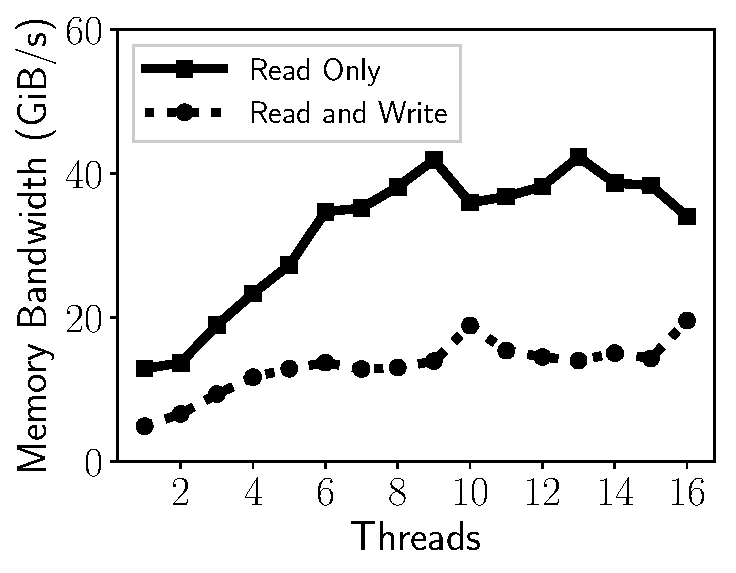
\includegraphics[width=0.33\textwidth, trim={0.5cm 0.5cm 0.5cm 1cm}]{figures/microbenchmarks_time_vs_threads.pdf}	
    \caption{Main memory bandwidth vs. the number of threads. Multiple threads are needed to saturate memory bandwidth. Simultaneous reading and writing has lower throughput than reading only.}
   \label{fig:mem_bandwidth_scalability}
\end{figure}

\end{description} 

\heading{Batched Predecessor Search}
   Let $A$ be a set of keys sorted in non-decreasing order,  
   where each key is denoted as $a_i$, where $i=1, 2,\ldots,n$, and $B$ be a set of queries sorted in non-decreasing order, 
   where each query is denoted as $b_j$, where $j=1, 2,\ldots,n$. For each query, $b_j\in B$, the batched predecessor search 
   finds the largest value of $i$, such that $a_i\leq b_j$. While $A$ and $B$ can vary in size, for simplicity, we assume $|A|=|B|=n$.

\heading{Multiway Merging}

   Given input array $A$ consisting of $k$ sublists, denoted as $S_j$, 
   where $j=1, 2,\ldots,k$, each of size  $\frac{n}{k}$ and sorted in non-decreasing order, we wish to output the $n$ total elements 
   in sorted order. Furthermore, we assume that $k$ is small enough that we can load elements 
   from each sublist into memory without degrading CPU cache utilization.

\heading{Partitioning}

Given an unsorted list, $A$, of $n$ elements, we wish to partition $A$ into $k$ buckets $A_1, A_2, \ldots, A_k$ of roughly equal size such that each bucket is value-disjoint.  That is, for any two elements $a \in A_i$ and $b \in A_j$, if $i < j$, then $a<b$. Partitioning involves $(i)$ finding pivots for each bucket ($k$ total); $(ii)$ determining which bucket each element is in; and, $(iii)$ moving each element into contiguous memory with other elements in the same bucket.  

  \end{block}

\end{column}

\separatorcolumn

\begin{column}{\colwidth}

  \begin{block}{Research Highlights}


\begin{figure}[htp]
\centering
\subfigure[Batched Predecessor Search, $\newline$ model: $f=0.54$.]{
    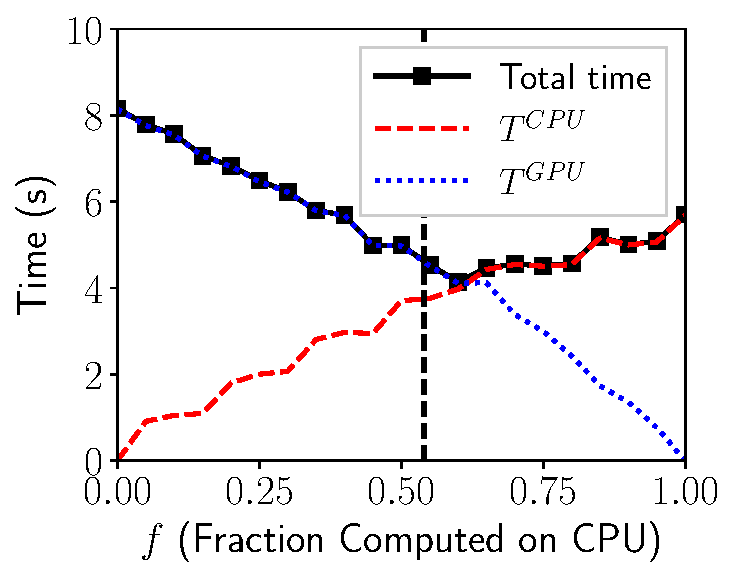
\includegraphics[height=0.20\textwidth, width=0.3\textwidth, trim={0.2cm 0.2cm 0.2cm 0.2cm}]{figures/time_vs_cpu_frac_predecessor.pdf}	
    }
\subfigure[Multiway Merge, model: $f=0.47$. $\newline$ We use $k=8$.]{
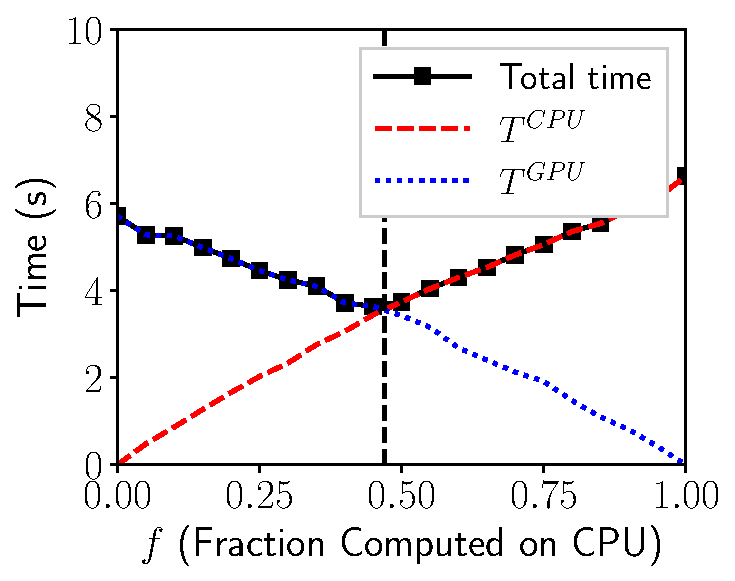
\includegraphics[height=0.20\textwidth, width=0.3\textwidth, trim={0.2cm 0.2cm 0.2cm 0.2cm}]{figures/time_vs_cpu_frac_multiway.pdf}}
\subfigure[Partitioning, model: $f=0.31$. $\newline$ We use $k=1024$ and $\mu=32$.]{
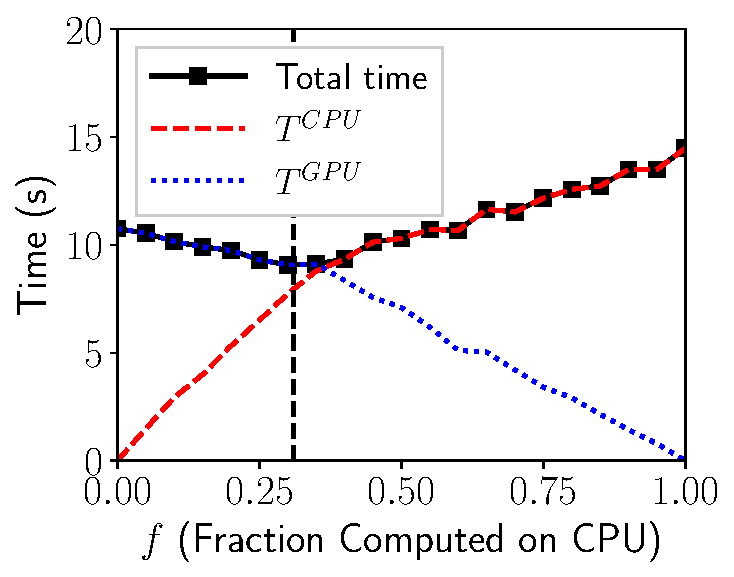
\includegraphics[height=0.20\textwidth, width=0.3\textwidth, trim={0.2cm 0.2cm 0.2cm 0.2cm}]{figures/time_vs_cpu_frac_partition.pdf}
}
%\captionsetup[figure]{font=small}
 \caption{Hybrid model accuracy for all algorithms. The total response time, $T^{CPU}$, and $T^{GPU}$ vs. $f$, are plotted. We show $n=4.0\times10^9$ for all algorithms. The vertical dashed line in each plot denotes the modeled value of $f$.}

 \label{fig:time_vs_f}
\end{figure}


\begin{description}[font=$\bullet$~\normalfont\scshape\color{red!50!black}]
\item  Figure 2(a) shows that even if the model can predict a good value for $f$, small differences in $f$ can yield significant load imbalance for the batched predecessor search. 
\item Figure 2(b) demonstrates that the optimal value of $f$ for multiway merging is almost exactly the value predicted by our model.
\item  Figure2(c) indicates that the model prediction is quite accurate, with the best performance achieved when $f=0.35$ being only slightly faster than the predicted value of 0.3.
\end{description}


%trim={0.2cm 0.2cm 0.2cm 0.2cm}
 \begin{figure}[htp]
\centering
\subfigure[]{
    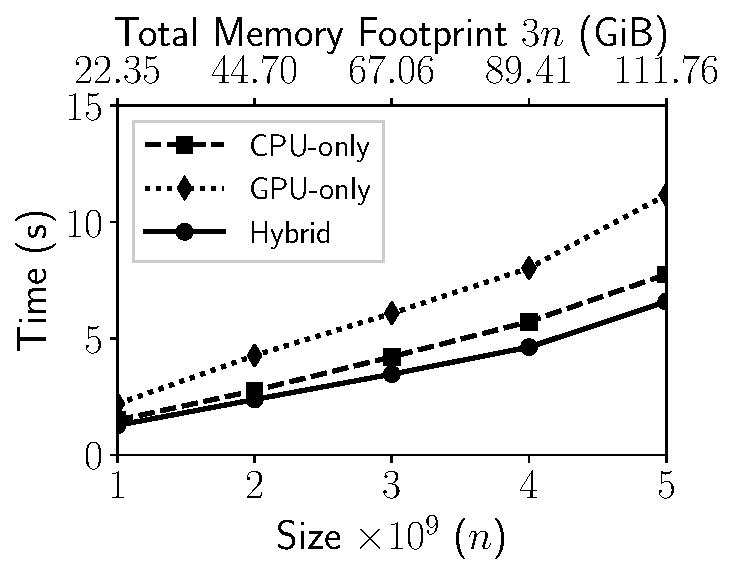
\includegraphics[width=0.31\textwidth, trim={0.2cm 0.2cm 0.2cm 0.2cm}]{figures/size_vs_time_predecessor.pdf}	
}
\subfigure[]{
    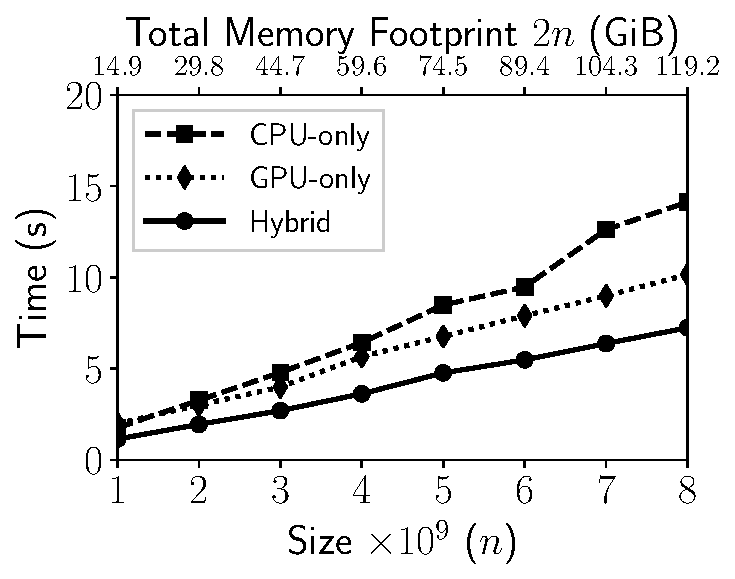
\includegraphics[height=0.20\textwidth, width=0.31\textwidth, trim={0.2cm 0.2cm 0.2cm 0.2cm}]{figures/size_vs_time_multiway.pdf}	
}
\subfigure[]{
    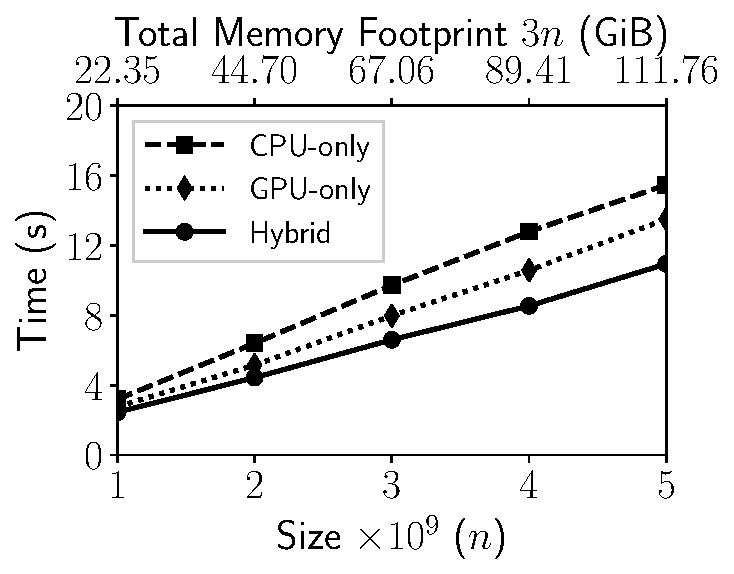
\includegraphics[height=0.20\textwidth, width=0.31\textwidth, trim={0.2cm 0.2cm 0.2cm 0.2cm}]{figures/size_vs_time_partition.pdf}	
}
    \caption{(a), (b), and (c) Response time vs. input size ($n$) comparing CPU-only, GPU-only, and hybrid batched predecessor, multiway merging, and partitioning algorithms, respectively.}
   \label{fig:predecessor_search_results}
\end{figure}
 

\begin{figure}[htp]
\centering
\subfigure[]{
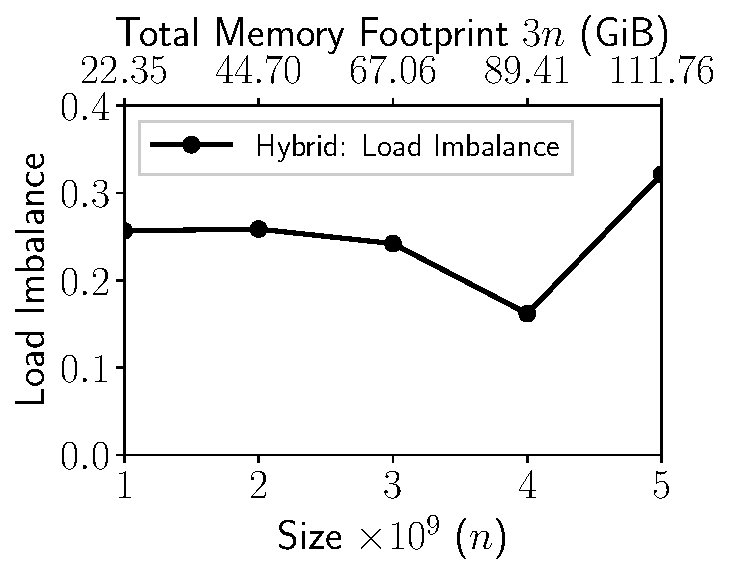
\includegraphics[width=0.31\textwidth, trim={0.2cm 0.2cm 0.2cm 0.2cm}]{figures/size_vs_load_imbalance_predecessor.pdf}	
}
\subfigure[]{
    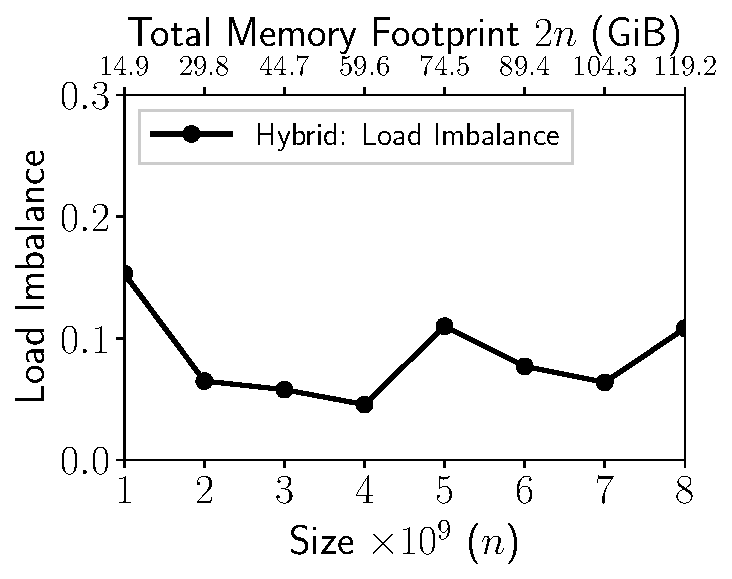
\includegraphics[height=0.20\textwidth, width=0.31\textwidth, trim={0.2cm 0.2cm 0.2cm 0.2cm}]{figures/size_vs_load_imbalance_multiway.pdf}	
}
\subfigure[]{
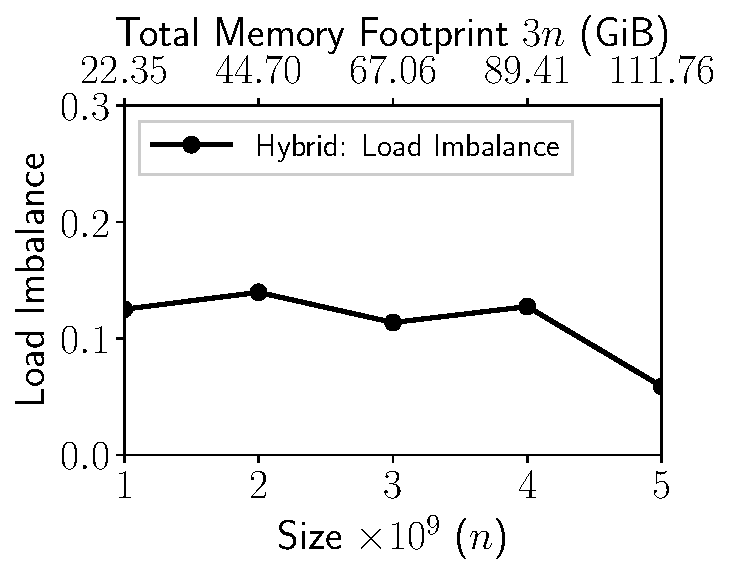
\includegraphics[height=0.20\textwidth, width=0.31\textwidth, trim={0.2cm 0.2cm 0.2cm 0.2cm}]{figures/size_vs_load_imbalance_partition.pdf}	
}
\caption{(a), (b), and (c) The load imbalance of the hybrid algorithms in Figure~\ref{fig:predecessor_search_results}(a), (b), and (c), respectively. }
\label{fig:multiway_merge_results}
\end{figure}

\end{block} 

\begin{block}{Future Work}

\begin{description}[font=$\bullet$~\normalfont\scshape\color{red!50!black}]
\item Investigating whether compression schemes or other memory transfer optimizations can alleviate some of the bottlenecks, despite the computational overhead.
\item The study of other fundamental database operations that have not been considered for GPU acceleration.
\end{description}

\end{block}

\begin{block}{Acknowledgements}
This material is based upon work supported by the National Science Foundation under Grant OAC-1849559 and Fonds de la Recherche Scientifique-FNRS under Grant no MISU F 6001 1.
\end{block}

\end{column}

\separatorcolumn
\end{columns}
\end{frame}

\end{document}
